%\documentclass[11pt, oneside]{article}   	
%\usepackage{geometry}    
%\geometry{letterpaper}                 		
\input preamble.tex
\newcommand{\ig}[2][width=4in]{\includegraphics[#1]{#2}}    		
\usepackage{graphicx}					
\usepackage{amssymb}
\usepackage{pgfplotstable}
\usepackage{float}
\usepackage{caption}
\captionsetup[table]{justification=justified,singlelinecheck=false, position=bottom}
\begin{document}

\header {\today}							
\title{Rutherford Scattering}
\author{Ekta "The Bomb" Patel \& Brandon Booth-Dunbar}

\section{Abstract}
\begin{em} In this lab, we verify the Rutherford formula for nuclear scattering in 1909. Their experiment led to the confirmation of the existence of an atomic nucleus, thus destroying the plum pudding model  developed by J. J. Thomson. Rutherford's team successfully disproved Thomson's model by observing a significant amount of charged alpha particles scattering back from a thin sheet of gold foil rather than passing through it with only a few deflections. Therefore, they were able to confirm that an atom consists of a dense nucleus surrounded by a less dense cloud of electrons surrounding the heavy nucleus, instead of an even distribution of mass throughout the atom. The distribution of alpha particles scattered by gold foil can be observed as a function of the scattering angle, which relies on the distance between the foil and the gold source. \end {em}

\section{Theory}
%B&E
Geiger and Marsden formed the first preliminary theory for the Rutherford model of the atom. They were able to gather that most $\alpha$-particles, He nuclei, passed right through a thin foil without being deflected. However, there were many particles that experienced large angle scattering. The differential scattering cross section will be determined in this lab: 
\begin{equation} \frac{d\sigma}{d\Omega}(\theta)\Delta\Omega=\frac{number\;of\; particles\; per\; unit\; time\;into\;a \;solid\; angle\; \Delta\Omega(\theta)}{(number \;of\; scatterers)\times (incident\; flux)} \end{equation}

Based on the previous definition, Rutherford was able to show that a positively charged nucleus has a differential scattering cross-section for charged particles that is given by:
\begin {equation}\label{scattering} \frac{d\sigma}{d\Omega}(\theta)= \frac{Z^2z^2e^4}{16E^2} \frac{1}{sin^4(\theta/2)}\end{equation} where $Ze$ is nuclear charge, $ze$ is charge of the scattered particle and $E$ is the energy of the scattered particle. $\theta$ is the scattering angle. However, we can see that this equation does not give appropriate units for a number of particles per area, instead we have $\frac{C^4}{J^2}$.
In order to correct this dimensional analysis disagreement, we look at the kinetic energy of the alpha particle, $E$, which is:
\begin{equation} E=\frac{1}{2}mv^2.\end{equation} However, when colliding alpha particles head on with the nucleus, all of the kinetic energy is turned into potential energy and the particle is at rest, so $E$ is also:
\begin{equation} E=\frac{q_1q_2}{4\pi\epsilon_0 b}.\end{equation} In the previous equation, $q_1=Ze$ and $q_2=ze$. We can solve for $b$, the distance between the center of the alpha particle and the center of the nucleus, where\begin{equation} b= \frac{Zze^2}{2\pi \epsilon_0 mv^2}.\end{equation}
Therefore, Equation \ref{scattering} can be rewritten as\begin{equation}\frac{d\sigma}{d\Omega}(\theta)=\left(\frac{1}{4b}\right)^2\frac{1}{sin^4(\theta/2)}.\end{equation}
\newline The scattering cross section can then be used to find the rate of detected particles, $N_2$, which is expressed in\ terms of $N_0$, the total number of particles emitted by the source per unit solid angle. Using the geometry of the set up and the Rutherford formula, the rate of detected particles is determined by the following formula
\begin{equation} N_2=n\frac{d\sigma}{d\Omega}(\theta)\Delta\Omega_2\times (incident\;flux)\end{equation} where $n$ is the number of scattering centers. The incident flux is given by $\frac{N_0}{R_1^2}$, which correspond to the figures in the next section. Then, $N_2$ is:
\begin{equation} N_2=\frac{nN_0}{R_1^2}\frac{d\sigma}{d\Omega}\Delta\Omega_2.\end{equation}
The scattering angle, $\theta$, varies with the changing distance $Y$ in the apparatus. Using the geometry of the setup, this formula can be given as
\begin{equation} \label{complicated}N_2=N_0\times \left( \frac{nA_2Z^2z^2e^4}{R_1^2r_1^2 16 E^2}\right)\times \left(\frac{cos\theta_2 sin\theta_2^2}{sin(\theta/2)^4}\right) \end {equation}\\or more simply as\begin{equation}  \label{simple}N_2=N_0\times G\times f(Y). \end{equation} Here G is the atomic factor that accounts for the force between the gold atoms and the scattered alpha particles as they pass through the gold foil. Here, we take for granted that the solid angles we mention are averages and that the scattering center is an average scattering center since we do not know where on the surface area of the gold foil each, or most, of the alpha particles will pass through. 
\section{Experimental Methods}
\subsection{Apparatus}
\indent \indent The experimental apparatus consists of a vacuum tube with a detector placed at one end and a plunger with a radioactive source placed at the other. the radioactive source used in this lab is Americium 241, it is highly radioactive so caution must be used at all times. The source can be moved over a range of roughly 20 cm in order to take measurements of scattering over a variety of scattering angles. It is important to note that moving the source over the 20 cm range is analogous to moving the detector over that range while leaving the source fixed.  The only reason that I point this out is because the lab manual for this experiment mixes up the source and detector multiple times.  To remain consistent with the resources given to us for this lab and the questions asked, including the results of Eq. 16 and Fig. 3, we will perform our analysis as though we are moving the detector.  This will not change our conclusion or results but will keep us consistent with the specific analysis asked for in the lab manual. The geometry of the figure is given below in Fig. 1 for reference.
 
\begin{figure}[H]
\begin{center}
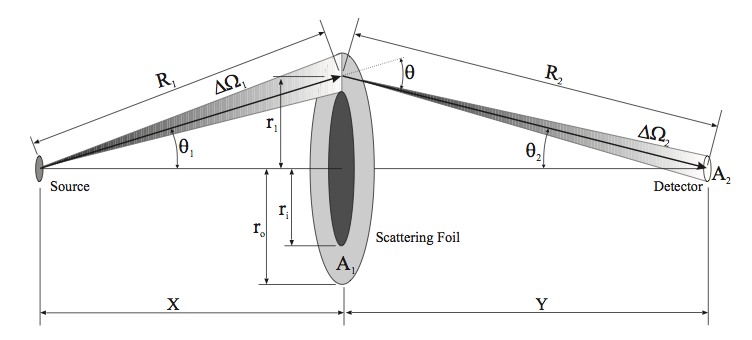
\includegraphics[width=7in]{apparatus.png}
\caption{Experimental geometry.}
\end{center}
\end{figure}

\indent \indent The vacuum tube is connected to a pump which maintains a negative pressure of 30 $\pm$ 0.1 psi while data is being taken.  The detector is connected first to a pre-amplifier which boosts the signal before its arrival at a linear amplifier.  The amplified signal is then given to a discriminator which does not accept signals below a certain voltage, the calibration for the discriminator is given in the following section.  If the signal meets the discriminator voltage requirement it will be forwarded to a counter and recorded. This simple signal path can be seen below in Fig. 2 for reference.    


\begin{figure}[H]
\begin{center}
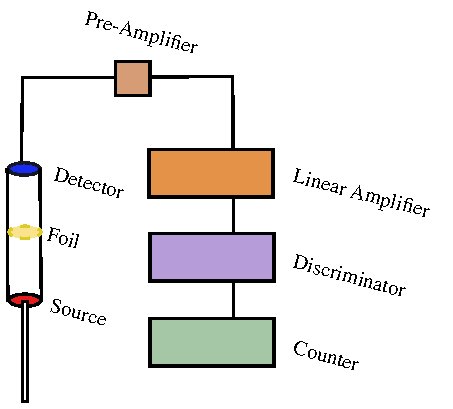
\includegraphics[width=4.5in, angle=90]{Figure1Ap.pdf}
\caption{Apparatus Signal Path}
\end{center}
\end{figure}

\subsection{Preliminary}
\indent \indent  Before beginning any experimentation there are three important things to keep in mind for the duration of the experiment. 
\begin{enumerate}
\item The source $^{241} Am$ is highly radioactive and should not be touched with bare hands or removed without proper tools and supervision. 
\item All electronics must remain off until the vacuum tube is brought to the required pressure.  The detector is held at a potential such that if it were to be turned on in the presence of the number of particles at regular air pressure the sensitivity would be damaged permanently.
\item When releasing the pressure from the vacuum tube (after turning off all the electronics) be very careful.  If the pressure is released too rapidly the rapid flow of air can not only tear the gold foil but also expunge radioactive debris from the source into the lab. 
\end{enumerate}

\subsection{Calibration \& Procedure}
\indent \indent  To begin the calibration we obtained the Bismuth 83 source from the instructor and placed it in the extra vacuum tube provided. After gently removing the detector from the primary vacuum tube we transferred it;  placing the $^{83}Bi$ source as far away from the detector as possible while ensuring that it was still retrievable. After bringing the tube to the required pressure we turned on the electronics.  From here we started with the discriminator at the lowest setting and took a count of 5 minutes.  Using this as our baseline we increases the threshold of the discriminator until we began to see a decrease in counts greater than $\sqrt{N}$ where N is the number of counts.  Surprisingly we never saw a noticeable decrease even after bringing the discriminator to the largest possible threshold.  Usually this is an indicator that the amplifier is set too high but this is only a problem if we are additionally recording large background counts.  To test this we removed the radioactive source and performed 5 minute background counts.  Surprisingly enough we detected no more than 4 background counts which is extremely small compared to average count numbers in the hundreds.  

\indent \indent Furthermore during this time the detector was horizontally placed, which subjects it to the maximum flux of cosmic ray background, which will be our primary source of interfering radiation.  In the experimental apparatus the detector will be place vertically and will therefore have even less exposure to background. Additionally the experimental tube is shielded more than the test tube used for calibration making the likelihood of recording background counts even smaller.  Since we could not calibrate the detector in the experimental tube and our experimental counts are all above 1000 we discount background as a source of error in our measurements since it would make up only a small fraction of a percent in our experimental counts.  

\indent \indent After calibrating the discriminator we replaced the detector in its original position and brought the tube to the required psi before restarting the electronics. 


\subsection{Recording Data}
\indent \indent Before recording any data plot the test function $f(Y)$ as given in Eq. 16 so that you can ensure that the data you are taking matches the theory.  We chose an increment of 1 cm for our first run then increased our resolution by taking a second run at a 0.5 cm offset from our first run.  i.e. our first run of data was at integer points 1, 2, 3, 4... while our second set was at 0.5, 1.5, 2.5, ... . Once we took enough data we ensured that it met the test function and did our second run.  While students in past years have taken counts for upwards of 40 minutes we saw no reason to do such a thing when counts are already above 1000 for 20 minute intervals.  

\indent \indent The only involved part of taking data is moving the plunger upon which the source is placed.  It is truly a two person process which even when done very carefully results in some uncertainty.  The plunger is held in place by a collar which you move every time you would like to start a new count.  A note of caution, the plunger is pulled inward by the pressure within the vacuum tube so ensure that you have a firm hold before removing the collar and adjusting its position. 

\section{Results and Discussion}
\subsection{The Scattering Angle Distribution}
Using Equations \ref{complicated} and \ref{simple}, solving for $f(Y)$ gives the angular distribution as a function of Y. We can plot $Y$ vs. $f(Y)$ for a range of 0 cm to 20 cm to get a curve that we can use to fit our experimental results. We solve for f(Y) in the following steps:
\begin{equation} f(Y)=\frac{cos\theta_2 sin\theta_2^2}{sin(\theta/2)^4} \end{equation} where
\begin{equation} \theta_1=tan^{-1}\left(\frac{r_1}{X}\right)\end{equation} and
\begin{equation} \theta_2=tan^{-1}\left(\frac{r_1}{Y}\right)\end{equation} and
\begin{equation} cos\theta_2=\frac{Y}{\sqrt{Y^2+r_1^2}} \end{equation} and
\begin{equation} sin\theta_2^2=\frac{r_1^2}{Y^2+r_1^2}, \end{equation} therefore:
\begin{equation} f(Y)= \frac{\frac{Y}{\sqrt{Y^2+r_1^2}} \frac{r_1^2}{Y^2+r_1^2}}{sin(0.5(tan^{-1}\left(\frac{r_1}{X}\right) + tan^{-1}\left(\frac{r_1}{Y}))\right)^4.} \end{equation}\\
We know the following quantities as they are given in the lab manual because we cannot open the apparatus and check them for ourselves:
\begin{table}[H]
\begin{center}
\begin{tabular}{|c|c|}\hline
Quantity & Description \\ \hline 
$r_s=0.32\pm0.01cm$ & radius of source\\ \hline 
$X=7.22\pm0.01cm$ & detector to plane of scattering foil\\ \hline
$r_i=2.30cm$ & radius of the inside of the scattering foil\\ \hline
$r_o=2.70cm$ & radius of the outside of the scattering foil\\ \hline
$r_d=0.48cm$ & radius of the detector\\ \hline
\end{tabular}
\caption{Several components of the apparatus that have been measured for us so that we do not have to disassemble the radioactive source.}
\end{center}
\end{table}
Plotting this function for f(Y) over an interval of 0 to 20cm, we have:
\begin{figure}[h!]
\begin{center}
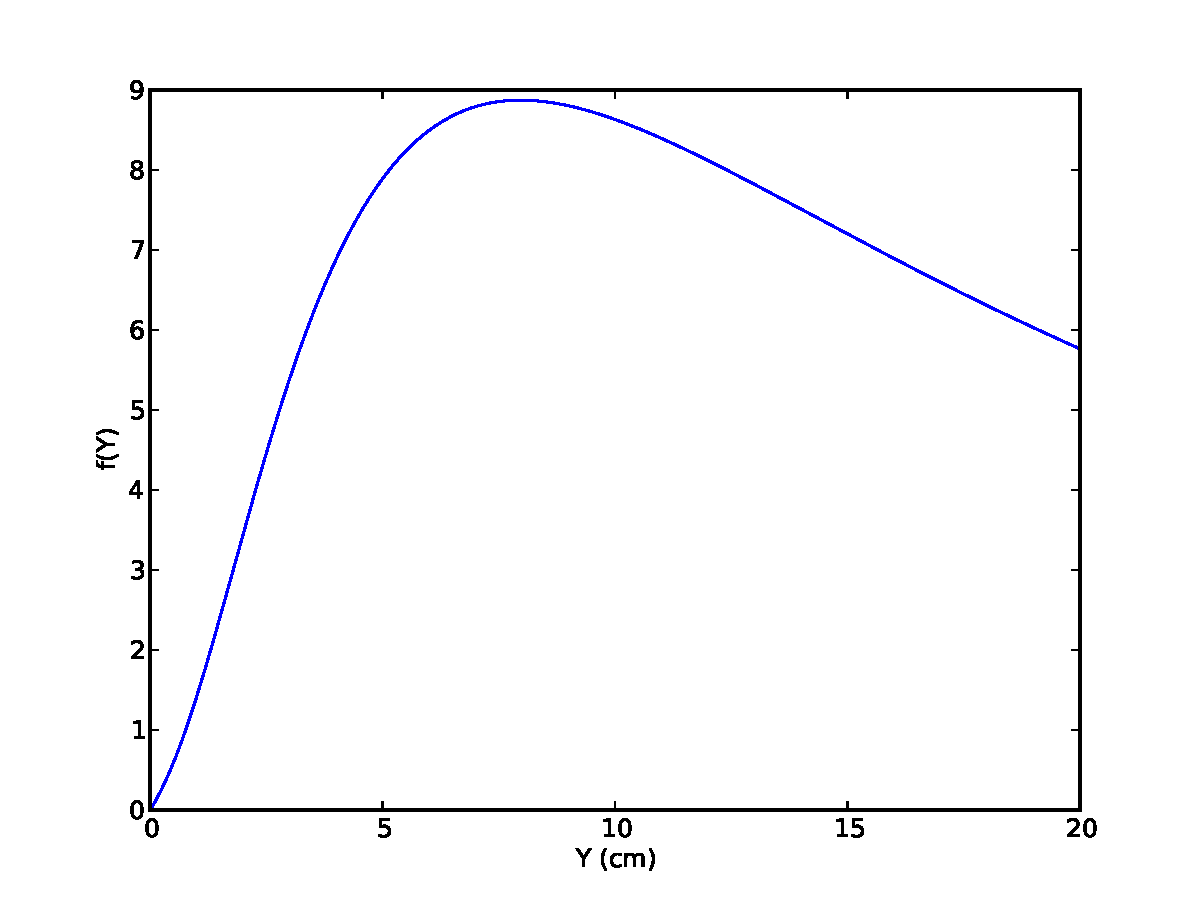
\includegraphics[width=4in]{preliminary_plot.pdf}
\caption{The angular distribution for the third term in the rate of detected particles($N_2$) that varies with the scattering angle as a function of length. The peak occurs in the vicinity of 8 cm.}
\end{center}
\end{figure}

\subsection{Determining $G$ \& $N_0$}
%EKTA FINISH THIS SECTION
Figure 3 below shows our preliminary data set taken over a range from 3cm to 18cm in 1cm intervals. At each value for Y, the distance from the gold foil to the source, we counted for 20 minutes. Our data shows a peak around 10cm as opposed to the 8cm prediction given in the angular distribution plot above. It can be seen however, that the peak distance is relative to where on the apparatus one begins to record data. The axis on which we can move the source in an out of the apparatus chamber was measured to be 19.7cm$\pm$.01cm long. The length along this axis at which we choose to begin measurements however, is dependent on our gains for the linear amplifier in the electronic schematic of the apparatus, and therefore arbitrary to the length at which we make our zero reference point. 
\begin{figure}[H]
\begin{center}
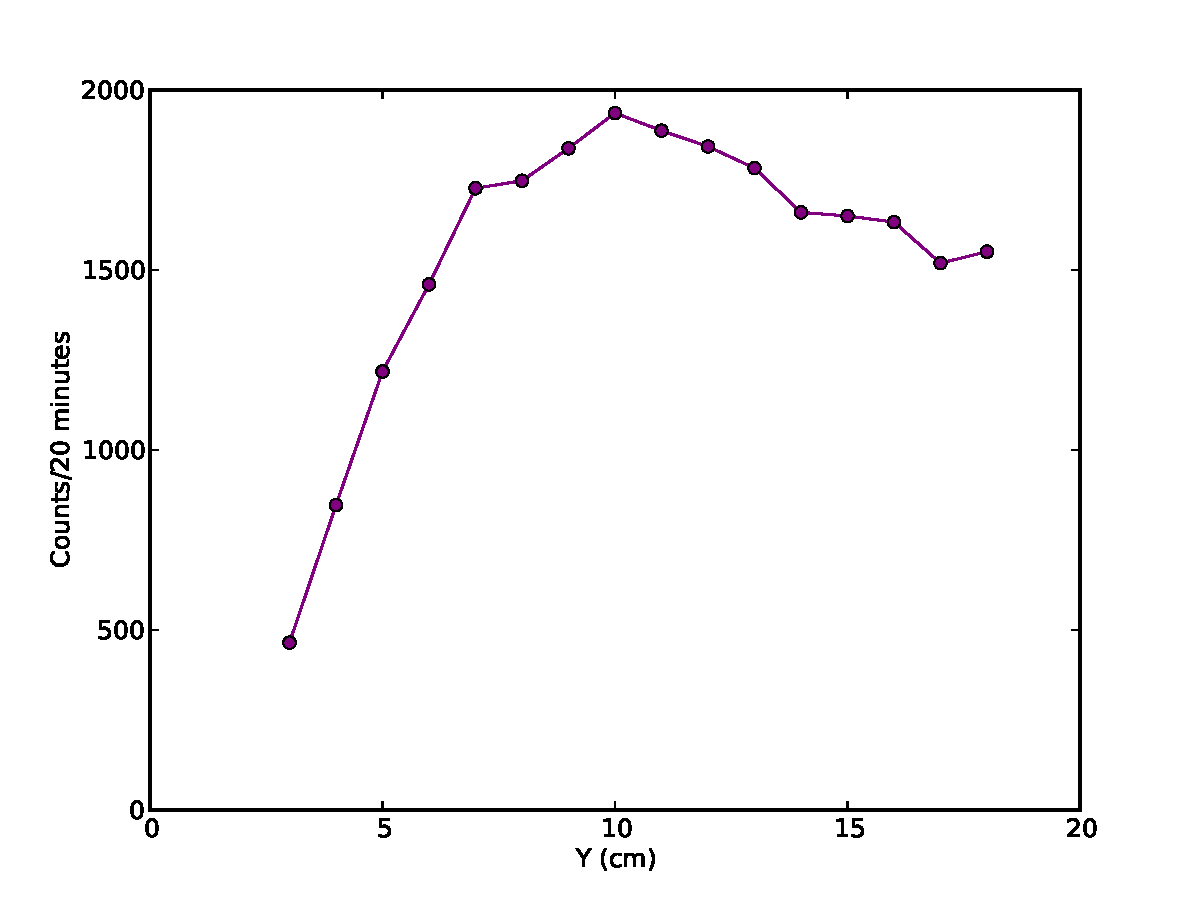
\includegraphics[width=4in]{firstrun.pdf}
\caption{The first run of data taken from 3cm to 18cm in intervals of 1cm.}
\end{center}
\end{figure}
After seeing a curve that represented the same shape as that of $f(Y)$, we went back and collected data in between the intervals we previously recorded so that we could have a full set of data from 3cm to 18cm in 0.5cm steps. 
\begin{figure}[H]
\begin{center}
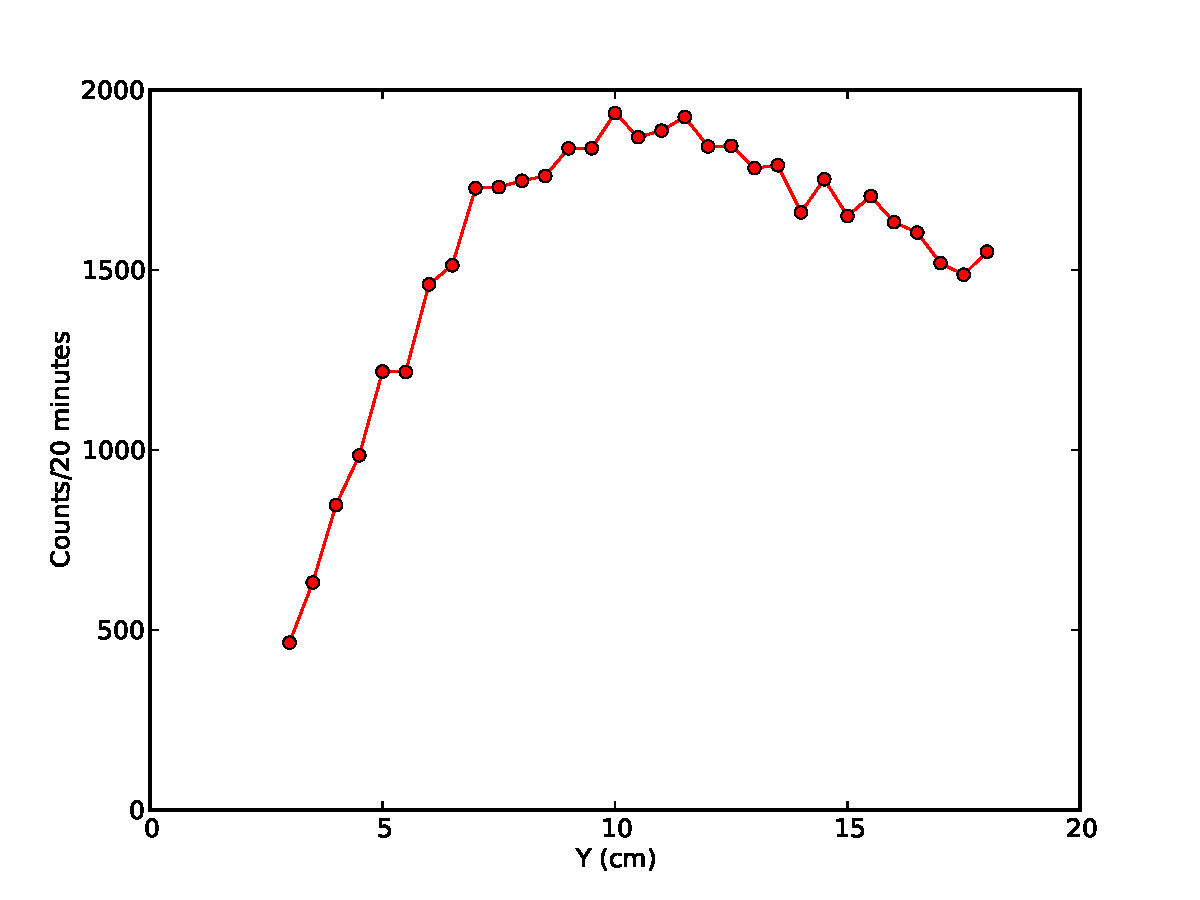
\includegraphics[width=4in]{secondrun.pdf}
\caption{The first run of data taken from 3cm to 18cm in intervals of 1cm combined  with an additional run with points taken in intervals of 0.5cm to obtain greater resolution.}
\end{center}
\end{figure}

Since we cannot find a value for $N_0$ directly because it would require dissembling the apparatus chamber and placing the detector directly next to the source, we can indirectly calculated it using the three values that we know or have measured, $G$, $N_2$, and $f(Y)$. First, G is simple a factor that is a result of combination of known values in this apparatus. 
\begin{equation}G=\frac{nA_2Z^2z^2e^4k^2}{R_1^2r_1^2  E^2}\end{equation}
That factors that are included in $G$ are listed below:

\begin{table}[H]
\begin{center}
\begin{tabular}{|c|c|c|}\hline
Quantity & Description & Value\\ \hline
 $n=\left(\frac{\rho N_A}{A_g}\right)A_1 t$ & Total number of scattering centers& $1.491\times10^{19}$ \\ \hline
 $\rho$ & Density of Gold &$1.93\times10^4 kg/m^3$ \\ \hline
$N_A$ & Avogadro's Number &  $6.022\times10^{23}$\\ \hline
$A_g$ & Atomic weight of Gold & $196.97 u= 0.197 kg/mol$ \\ \hline
$A_1=\pi r_o^2-\pi r_i^2 $ & Area of scatting foil& $1.257\times10^{-4} m^2$ \\ \hline
 $t$ & Thickness of scattering foil & $2\times10^{-6} m$\\ \hline
$A_2=\pi r_d^2$ & Area of the detector & $1.508\times10^{-4}m^2$\\ \hline
$Ze$ & Nuclear charge &$79\times (1.6\times^10^{-19} C)$\\ \hline
$ze$ & Alpha particle charge & $2\times(1.6\times^10^{-19} C)$\\ \hline
$E$ & Energy of scattered particle &$4.4MeV=7.0496\times10^{-13}J$\\ \hline
$R_1$ & Hypotenuse from source to scattering foil& $0.03118m$\\ \hline
$r_1$ & Average scattering center & $0.025 m$ \\ \hline
$k$ & Coulomb's constant & $9\times10^9 N\cdot m/ C^2$\\ \hline

\end{tabular}
\caption{All values needed to calculate the factor G as given by the lab manual and the period table.}
\end{center}
\end{table}
Therefore, $G=8.932\times10^{-6}$. We cannot propagate error on the value for $G$ because the values that we are using are taken for granted since we cannot make our measurements of the apparatus that are inside the chamber. We can now use the calculated value for $G$, the angular distribution $f(Y)$ and the experimentally collected count rates, $N_2$ to determine $N_0$. 
\begin{equation} N_0=\frac{N_2}{f(Y)G}= 2.2509\times10^7\pm4.8028\times10^6\;particles/20\;minutes\end{equation} 
Here we calculate the standard deviation by the following formula:
\begin{equation} \sigma_{N_0}=\sqrt{\frac{1}{N}\Sigma (N_{average} - N_i)}=4.8028\times10^6\;particles/20\;minutes\end{equation}
The value for $N_0$ should hypothetically be much higher than the values for $N_2$ that we are experimentally measuring because $N_0$ is the number of particles that the source is emitting directly, which is much more than what we measure for the counts as a function of distance from the source. Since the zero reference point of the length is arbitrary, we shift our length values by two centimeters to the left to arrive at results that correspond to our calculated curve. The most important comparison is how optimally our data follows the calculated curve, not how in or out of phase the curves are themselves. 

%%%%% error propagation

\begin{figure}[H]
\begin{center}
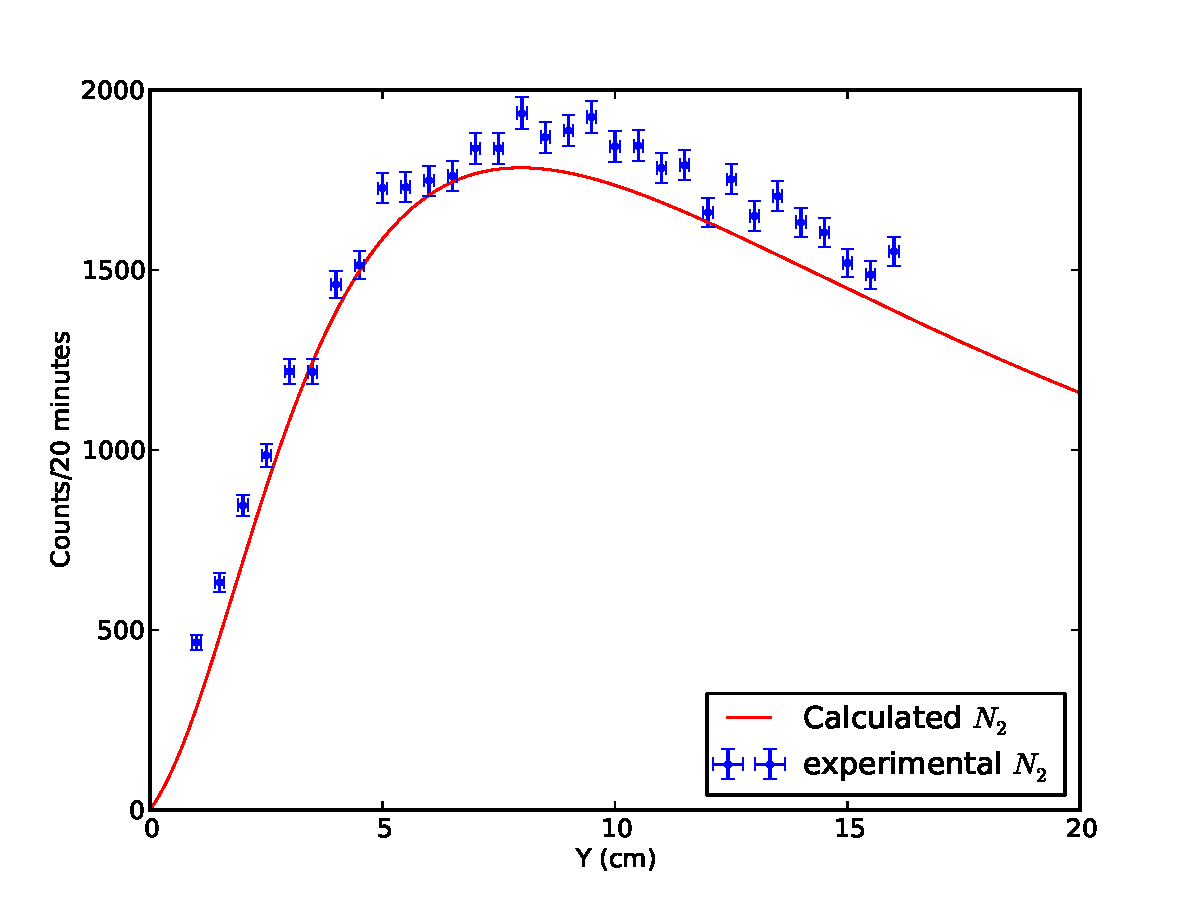
\includegraphics[width=5in]{N2.pdf}
\caption{The calculated value for $N_2$ is shown in red, while our experimental value for $N_2$ is given in the blue data points with error bars corresponding to $\sqrt{\#\; of\; counts}$ per data point.}
\end{center}
\end{figure}
Our experimental values tend to vary from the calculated rate of scattered particles mostly after the peak of the curves, which are about the same. The reason for this discrepancy at higher values for $Y$ is due to the fact that there is a higher chance of particles scattering off of the walls of the chamber and still making it though to the detector. Therefore, there is some over-counting that we see at values of $Y$ greater than about 8cm.

\subsection{Finding the Atomic Number ($Z$)}
The atomic number of gold, given by $Z$, cannot be found using our data because we would need to disassemble the apparatus and place the source right next to the detector in order to determine the proper value for $N_0$. $Z$ is a factor in $G$, so when we rearrange Equation \ref{simple} appropriately, we have: 
\begin{equation}G(Z)= \frac{N_2}{N_0 \times f(Y)}. \end {equation} 
In the above equation, we have values for $N_2$ and a distribution to represent $f(Y)$, but if we cannot experimentally determine $N_0$,  we do not have enough known variables to solve for $Z$. Therefore, we accept that the atomic number of Gold is 79 as given by the periodic table. 
\subsection{Calculating the Nuclear Radius Upper Limit}
The upper limit of the nucleus radius can be determined from the impact parameter, $b$, which we derived earlier in section 2. It is the distance from the center of the alpha particle to the center of the nucleus. The alpha particles do not have enough force to penetrate the nucleus a significant amount compared to the radius of the nucleus, so even though $b$ is the sum of the alpha particle radius and the nucleus radius, we can assume that it is a good approximation for the upper limit of the nuclear radius. Therefore, we know that $b$ is: \begin{equation} \label{b}b= \frac{Zze^2}{2\pi \epsilon_0 mv^2}.\end{equation} Here, we are also making the assumption that the alpha particles hits the nucleus head on and deflects back along a straight line 180$^\circ$ from its initial impact. The quantities in Equation \ref{b} are:
\begin{itemize}
\item $Ze=79\times (1.6\times^10^{-19} C)$
\item $ze= 2\times(1.6\times^10^{-19} C)$
\item $\frac{1}{4\pi\epsilon_0}=9\times10^9 N\cdot m/ C^2$
\item $m=6.7\times10^{-27} kg$
\item $v=2\times 10^7 m/s$
\end{itemize}
Therefore, \begin{equation} b= \frac{(79\times (1.6\times^10^{-19} C))(2\times(1.6\times^10^{-19} C))(9\times10^9 N\cdot m/ C^2)}{(6.7\times10^{-27} kg)(2\times 10^7 m/s)^2}=2.7\times10^{-14}m.\end{equation}
The upper limit on the nuclear radius of Gold is $2.7\times10^{-14}$m as calculated from the parameters given the setup that we have for this experiment.


\section{Conclusion}
\subsection{Review of Results}
\indent \indent Overall our results were very good with only slight deviation from expected values.  Our experimental data does not exactly match the calculated scattering curve which is most likely a result of our inability to accurately move the plunger.  While we did our best there are no markings on the plunger and it is difficult to tell how far you have really moved.  This is most likely the source of our seemingly symmetric drift above the calculated number of counts.
\indent \indent  Outside of the error caused by the plunger we did not find any significant deviations in our data from what is to be expected and our results overall very much reflected the experimental goals set out in the lab manual.

\subsection{Suggested Improvements}
\indent \indent First and foremost, mark the plunger so that it is much easier to reliably measure the distance axis on our data.  While our official error is only 0.1 cm the real error caused by simple human clumsiness is most likely much greater.  The only other improvement that would be useful is to either make the foil more easily removable or make the test tube a more accurate representation of the experimental tube so that a reliable background can be taken. 

\begin{thebibliography}{99}
\bibitem{electron}Sleator, Tycho, and Windt, David, \begin{em}Rutherford Scattering. \end{em}Experimental Physics. V85.0112. Spring, 2011.
\end{thebibliography}

\section{Appendix}
\begin{table}[H]
\begin{tabular}{|c|c|}\hline
Y (cm) & Counts/ 20 min\\ \hline
3.0 & 465  \\ \hline
4.0 &  847 \\ \hline
5.0 &  1218 \\ \hline
6.0 &  1460 \\ \hline
7.0 &  1727\\ \hline
8.0 &  1748 \\ \hline
9.0 &  1838\\ \hline
10.0 &  1936\\ \hline
11.0 &  1867\\ \hline
12.0 &  1843\\ \hline
13.0 &  1783\\ \hline
14.0 &  1660\\ \hline
15.0 &  1650\\ \hline
16.0 & 1633 \\ \hline
17.0 &  1519\\ \hline
18.0 &  1551\\ \hline
\end {tabular}
\caption{First run of data taken from 3cm to 18cm in intervals of 1cm.}
\end{table}

\begin{table}[H]
\begin{tabular}{|c|c|}\hline
Y (cm) & Counts/ 20 min\\ \hline
3.5 & 632 \\ \hline
4.5 &  985 \\ \hline
5.5 &  1217 \\ \hline
6.5 &  1513 \\ \hline
7.5 &  1730\\ \hline
8.5 &  1741 \\ \hline
9.5 &  1838\\ \hline
10.5 &  1869\\ \hline
11.5 &  1925\\ \hline
12.5 &  1845\\ \hline
13.5 &  1791\\ \hline
14.5 &  1752\\ \hline
15.5 &  1705\\ \hline
16.5 & 1604\\ \hline
17.5 &  1487\\ \hline
\end{tabular}
\caption{Second run of data taken from 3.5 cm to 17.5cm in intervals of 1cm.}
\end{table}

\end{document}


